\chapter{Theoretical Foundation}

In this chapter, we want to give an overview of the theoretical foundations of manifolds, their learning task, and different methods designed to learn those manifolds. Afterward, we will introduce the concept of clustering and algorithms, which will be necessary for one aspect of our experiments later on.

\section{Manifold}

One can look at Fig. \ref{fig:1-dimensional_manifold} to understand the concepts of manifolds. There a 1-dimensional object in 3-dimensional space is depicted. This object has no volume or area that could be measured, so it can be considered a 1-dimensional line. If we now bend this line into a straight one, it can easily fit into a 1-dimensional space (Fig. \ref{fig:homeomorphism_line}). By doing so, one can conclude that the line has an \textit{extrinsic dimensionality} of 3 and an \textit{intrinsic dimensionality} of 1. The first describes the dimensionality that the object is initially represented in, and the latter describes the dimensionality that can be reduced to without losing much or, in this case, no information. This reduced object is then called a  1-dimensional manifold. One could also see that this object is a 1-dimensional manifold by not bending it but by zooming into the object. This leads to the perception of a 1-dimensional line (Fig. \ref{fig:zoom_in}). \cite{Cayton05}
\begin{figure}[!]
	\centering
	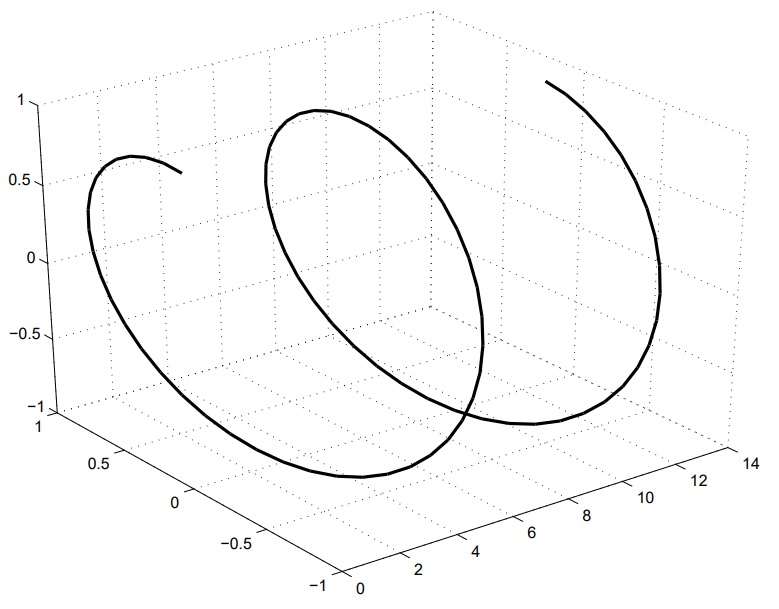
\includegraphics[width=\columnwidth-5cm]{images/1-dimensional_manifold.jpg}
	\caption[1-Dimensional Manifold]{1-Dimensional Manifold embedded in 3-Dimensional Space adapted from Fig. 2 in \cite{Cayton05}}
    \label{fig:1-dimensional_manifold}
\end{figure}
\begin{figure}[!]
	\centering
	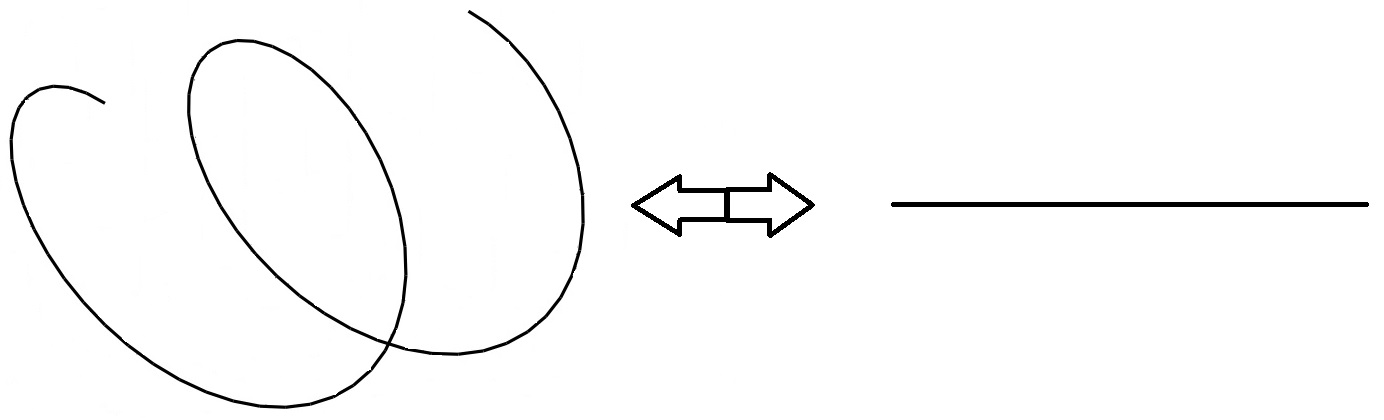
\includegraphics[width=\columnwidth]{images/homeomorphism_line.jpg}
	\caption[Bending a line]{Bending a line}
    \label{fig:homeomorphism_line}
\end{figure}
\begin{figure}[!]
	\centering
	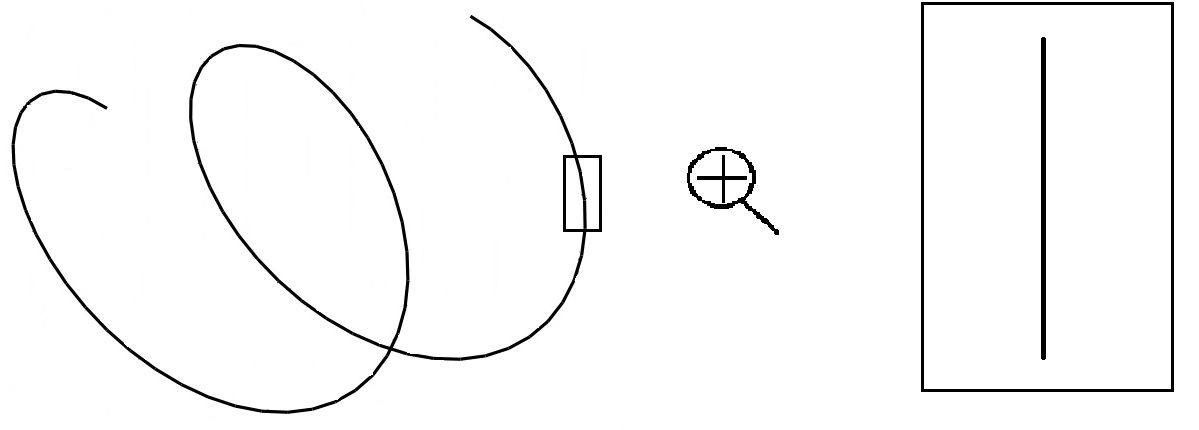
\includegraphics[width=\columnwidth]{images/zoom_in.jpg}
	\caption[Zooming into a line]{Zooming into a line}
    \label{fig:zoom_in}
\end{figure}

After giving an intuitive view of manifolds, we want to dive deeper into their formalisms. First, we introduce the notion of a \textit{topological space}. This geometric space is the most general type of space in which a notion of closeness is defined, but it can not be measured by a metric. The pair $(X, \mathcal{N})$ is called a topological space where $X$ is a set of elements (points) and the function $\mathcal{N}$ is the structure called topology which maps each element $x \in X$  to the set $\mathcal{N}(x) \subseteq X$. This set $\mathcal{N}(x)$ can be interpreted as a set of neighborhoods from $x$. \cite{wiki_topological_space}

Given a topological space, this can then be perceived as a specific shape. Transforming this shape by bending, stretching, squeezing, or shrinking leads to a new shape. From a mathematical standpoint, this new shape is no different from the old one because they both exhibit the same topological properties. This is demonstrated in Fig. \ref{fig:homeomorphism_line} where a spiral is bent into a line or in Fig. \ref{fig:homeomorphism} where a cube is inflated by pumping air into it, resulting in a sphere with no sharp edges and vertices. Those topological spaces are then called \textit{homeomorphic} because you can transform one space into another one without altering the topological properties. If topological spaces are homeomorphic, there exists a \textit{homeomorphism} between them which is a continuous function $f: X \to Y$ whose inverse $f^{-1}$ is also continuous. \cite{wiki_homeomorphism}
\begin{figure}[!]
	\centering
	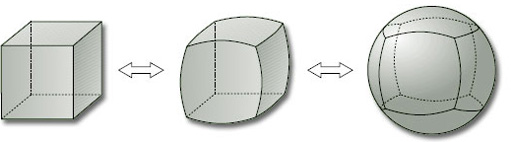
\includegraphics[width=\columnwidth]{images/homeomorphism.jpg}
	\caption[Demonstration on Homeomorphism]{Demonstration on Homeomorphism: Inflating a cube adapted from Fig. 39 in \footnotemark}
    \label{fig:homeomorphism}
\end{figure}
\footnotetext{\url{https://www.open.edu/openlearn/science-maths-technology/mathematics-statistics/surfaces/content-section-2.4}}

With this prior knowledge of topological spaces and homeomorphisms, we can now introduce the notion of manifolds. A \textit{d-dimensional manifold} $\mathcal{M}$, short \textit{d-manifold}, is a topological space in a lower dimension that is embedded into an artificially higher dimensional space. This higher dimension is the space $\mathbb{R}^D$ where $D$ is the dimensionality of that space with $d<D$. There then exists a local homeomorphism $f: \mathcal{N}(x) \to \mathbb{R}^d$ from the neighborhoods $\mathcal{N}(x) \subseteq \mathbb{R}^D$ of all the elements $x \in$ $\mathcal{M}$ in higher dimensional space to the lower dimensional space $\mathbb{R}^d$. This definition of a manifold is illustrated in Fig. \ref{fig:manifold}. \cite{Cayton05}
\begin{figure}[!]
	\centering
	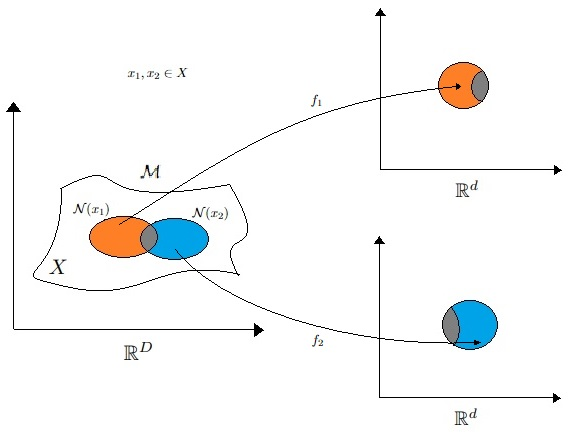
\includegraphics[width=\columnwidth]{images/manifold.jpg}
	\caption[Illustration of a Manifold and Homeomorphisms]{Illustration of a Manifold $\mathcal{M}$ and Homeomorphism $f_1$ and $f_2$, adapted from \cite{wiki_atlas}}
    \label{fig:manifold}
\end{figure}

One can then reconstruct the complete manifold in $\mathbb{R}^d$ the so-called \textit{Euclidean space}. This can be achieved by embedding all regions of the manifold into the Euclidean space. Those regions are specified by the homeomorphisms $f$ and are also called \textit{charts}, defined by the pair $(\mathcal{N}(x),f(x))$. The result of applying the first function is called \textit{domain}, and the application of the latter is called \textit{coordinates}. If we now have a collection of charts on $\mathcal{M}$, we get an \textit{atlas}. The formal definition of an atlas is \cite{wiki_atlas}
\begin{equation}
    \bigl\{ (\mathcal{N}(x),f(x)): x \in X \bigr\}
\end{equation}
and it has the property that it is fully covering the manifold $\mathcal{M}$ \cite{wiki_atlas}
\begin{equation}
    \bigcup_{x\in X}\mathcal{N}(x) = \mathcal{M}.
\end{equation}

Now that we understand the concept of a manifold, we can formalize the task of manifold learning.

\section{Manifold Learning}

For the task of learning a manifold $\mathcal{M}$, we assume that the manifold lies in a lower dimensional space that is embedded into an artificially higher dimensional space. We want to find an appropriate representation of this manifold in low dimensional space, meaning we want to uncover the intrinsic dimensionality of the manifold. Therefore the following problem is being solved in manifold learning. \cite{Cayton05}

\begin{task}
    \textit{Find coordinates} $y_1,...,y_n \in \mathbb{R}^d$ \textit{from data points} $x_1,...,x_n\in \mathcal{M} \subseteq \mathbb{R}^D$ \textit{where a single chart} $f: \mathcal{M} \to \mathbb{R}^d$ \textit{exists and the following holds:} $\forall i \in \{ 1,2,...,n \} : y_i=f(x_i)$.
\end{task}

This task of learning a manifold is necessary for analyzing high dimensional data and can be done by different manifold learning methods, as the name suggests. Therefore we want to take a closer look at those methods.

\section{Manifold Learning Methods}

Manifold learning methods are a family of dimensionality reduction techniques that aim to preserve the intrinsic structure of data and visualize it in a lower dimension space without losing most and, in the best case, no vital information. Furthermore, those methods are just concerned about nonlinear relations in the dataset other than linear dimensionality reduction methods. There will be three methods that we will introduce in the order of development date, namely Multidimensional Scaling (MDS), Locally Linear Embedding (LLE), and t-Distributed Stochastic Neighbor Embedding (t-SNE). They all have different characteristics and main focuses. For example are some of those parametric, which means that they need a parameter in order to be deployed, or some will try rather preserve more global than local structures or vice versa. As they have certain characteristics and main focuses, they also have specific limitations that we will elaborate on. This leads to advantages and disadvantages, and therefore they may be more suitable for specific contexts or data types.

\subsection{Multidimensional Scaling (MDS)}

"Multidimensional Scaling" is one of the oldest manifold learning methods, proposed by Torgerson in 1958 \cite{Torgerson52}. The idea is to reconstruct a lower dimensional embedding from high dimensional input data by preserving the pairwise similarities or distances from all points. Over the years, three different categories of variations of MDS were developed. One of which is \textit{classic MDS}. This variation is a linear dimensionality reduction method that aims to preserve the points' similarities measured by the \textit{inner product}. The inner product for points is defined as
\begin{equation}
   \langle x_i, x_j \rangle = \langle (x^1_i,...,x^D_i), (x^1_j,...,x^D_j) \rangle = x^1_i x^1_j + ... + x^D_i x^D_j 
\end{equation}
where the initial dimension $D$ is the input dimensionality. For the similarity measurement in the embedded space, one can replace $D$ with $d$ and $x_i, x_j$ with $y_i, y_j$. With this prior knowledge, we continue with the cost function that has to be minimized to obtain the embedding in the lower dimension
\begin{equation}
    \sum_{i<j} (\langle x_i,x_j\rangle - \langle y_i,y_j\rangle)^2.
\end{equation}
Furthermore, it was shown that classic MDS, also called \textit{Principle Coordinates Analysis (PCoA)}, is equivalent to PCA. \cite{ghojogh20} Another category of MDS is \textit{metric MDS}, which has an opposite view because it tries to preserve the pairwise distances instead of the similarities. In metric MDS, the cost function is also called \textit{stress function}
\begin{equation}
    \sqrt{\sum_{i<j} (d_x(x_i,x_j) - d_y(y_i,y_j))^2}
\end{equation}
where $d_x: \mathbb{R}^D \rightarrow \mathbb{R}$ and $d_y: \mathbb{R}^d \rightarrow \mathbb{R}$. By default, both metrics are Euclidean, but for $d_x$, any other valid metric could be chosen. The metric MDS is much slower than the classic MDS. It has the trade-off that it can now capture nonlinear structures but no longer has a closed form that could be easily calculated. Instead, metric MDS needs to be optimized iteratively. The third and last category of MDS is \textit{non-metric MDS} which considers the order or rank of distances of points in the embedded space instead of the distances themselves. For this purpose, a monotonic function $f(d_y(y_i,y_j))$ is defined, which maps the distances to ranks. The following equivalence expression shows the property that has to be fulfilled by the function
\begin{equation}
    d_y(y_i,y_j) \leq d_y(y_k,y_l) \Longleftrightarrow f(d_y(y_i,y_j)) \leq f(d_y(y_k,y_l)).
\end{equation}
In non-metric MDS, the following cost function is minimized
\begin{equation}
    \sqrt{ \frac{\sum_{i<j} (d_x(x_i,x_j) - f(d_y(y_i,y_j)))^2}{\sum_{i<j} d_x(x_i,x_j)^2}  }.
\end{equation}
[\cite{ghojogh20}, \cite{sorzano14}, \cite{Gisbrecht15}]
A visual illustration of how MDS reduces dimensions and tries to preserve distances is shown in Fig. \ref{fig:mds_illustration}.
\begin{figure}[!]
     \centering
     \begin{subfigure}[t]{\columnwidth}
         \centering
         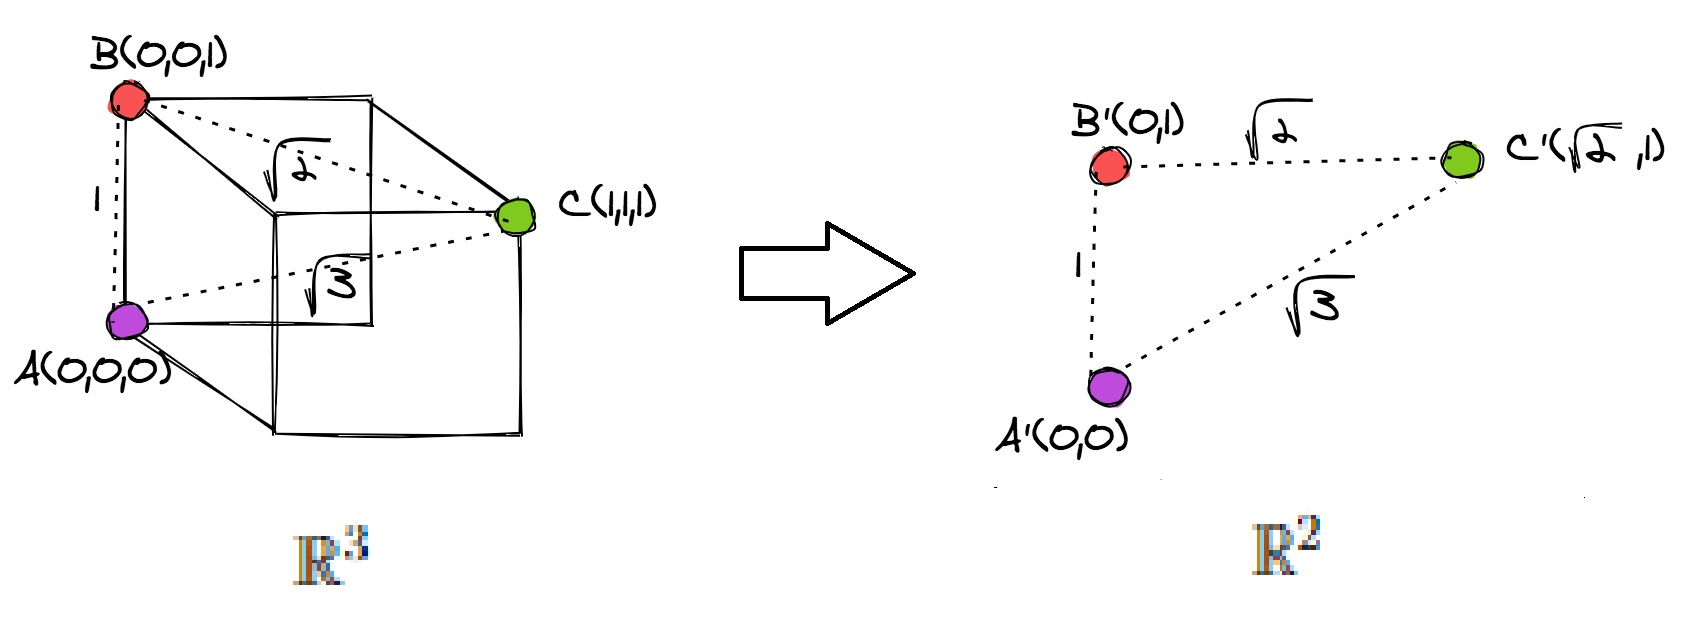
\includegraphics[width=\columnwidth]{images/mds_3D_2D.jpg}
         \caption{Mapping from 3D to 2D. The distances are perfectly preserved.}
         \label{subfig:mds_3D_2D}
     \end{subfigure}
     \hfill
     \begin{subfigure}[t]{\columnwidth}
         \centering
         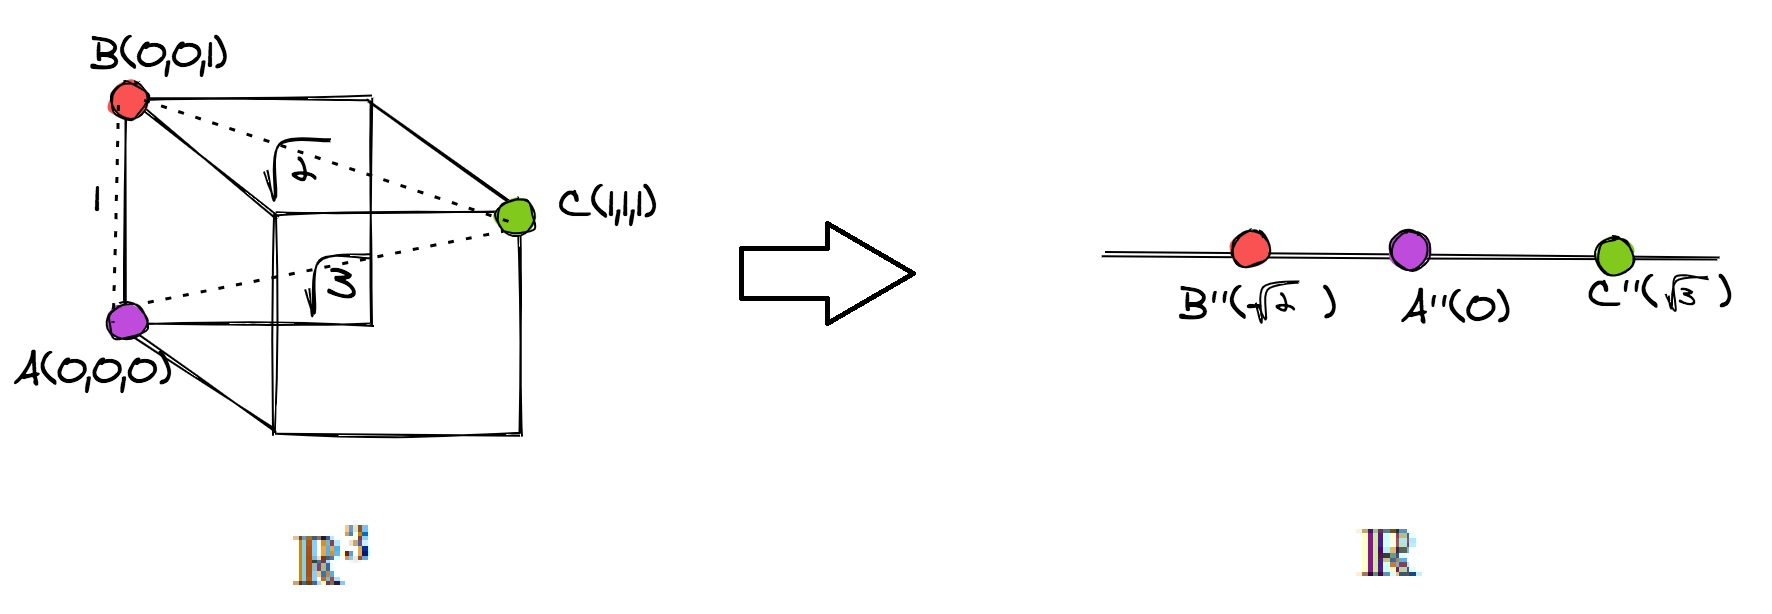
\includegraphics[width=\columnwidth]{images/mds_3D_1D.jpg}
         \caption{Mapping from 3D to 1D. The distances could not be preserved.}
         \label{subfig:mds_3D_1D}
     \end{subfigure}
        \caption[Illustration of MDS]{An illustration of MDS trying to preserve distances adapted from \footnotemark}
        \label{fig:mds_illustration}
\end{figure}
\footnotetext{\url{https://stackabuse.com/guide-to-multidimensional-scaling-in-python-with-scikit-learn/}}

\subsection{Locally Linear Embedding (LLE)}

The method "Locally Linear Embedding" was proposed by Roweis and Saul in 2000 \cite{saul00}. It has the innovation of recovering global structures by only looking at local structures. Those local structures, in our case called domain patches, are combined in an overlapping manner into a whole manifold. This leads to a neighborhood preserving property. The method consists of 3 steps, as shown in Fig. \ref{fig:lle_pipeline}. In the first step, the k-nearest-neighbors $\mathcal{N}_k$ of a point $x_i$ must be found. This shows that LLE is a parametric method that needs the parameter neighborhood size k before computation. Another way could be to choose the nearest-neighbors with the parameter of a fixed radius $\epsilon$. For those needed distance measurements, the Euclidean distance is being used. The second step of the method is to characterize the linear patches by representing $x_i$ as a weighted, convex combination of its nearest neighbors, meaning a linear combination where all coefficients are non-negative
\begin{equation}
    x_j \in \mathcal{N}_k(x_i) \Rightarrow W_{ij} \neq 0
\end{equation}
and they all sum up one 
\begin{equation}
    \sum_j W_{ij}=1.
\end{equation}
Another constraint to those linear combinations is that if a point $x_j$ is not a neighbor of $x_i$, the weight must be zero
\begin{equation}
    x_j \notin \mathcal{N}_k(x_i) \Rightarrow W_{ij}=0.
\end{equation}
This equation shows us that LLE is a local structure preserving method because it just considers the nearest neighbors of a point. To find the suitable reconstruction weight matrix, the following cost function, also called least-squared, is minimized
\begin{equation}
    \sum_i \norm{x_i - \sum_j W_{ij}x_i}^2.
\end{equation}
The weight matrix $W_i$ portrays the local geometry, or rather the structure, of a point $x_i$.
The third step is to construct the low dimensional embedding $y_i$ for the corresponding $x_i$ through the weight matrix $W$ that was determined in the previous step by minimizing the following cost function
\begin{equation}
    \sum_i \norm{y_i - \sum_{j} W_{ij}y_j}^2.
\end{equation}
with respect to $y_1,...,y_n$ instead of $W$, as in the previous step. Note that the embedding construction is only determined by the weight matrix and not from the initial inputs $x_1,...,x_n$. The weight matrix sort of saved the needed geometric encodings from the inputs. [\cite{saul03}, \cite{Cayton05}, \cite{Sarveniazi14}, \cite{Gisbrecht15}]
\begin{figure}[!]
	\centering
	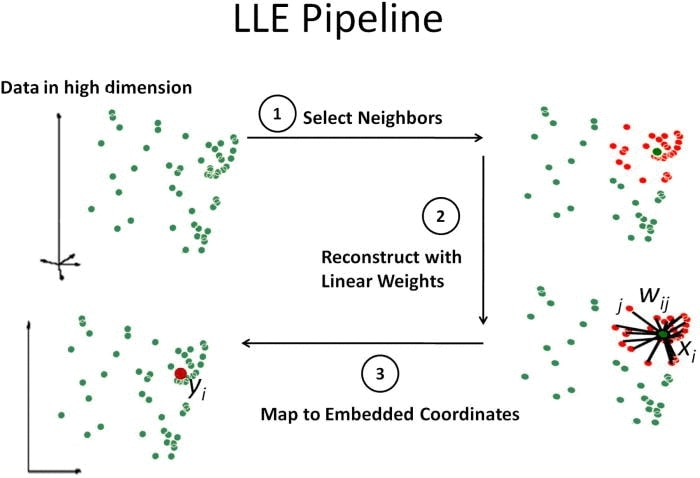
\includegraphics[width=\columnwidth]{images/lle_pipeline.jpg}
	\caption[LLE Pipeline]{LLE Pipeline in 3 steps adapted from Fig. 2 in \cite{Akhbardeh12}}
    \label{fig:lle_pipeline}
\end{figure}
Fig. \ref{fig:lle_illustration} shows visually how LLE reconstructs $y_i$ in the third step of the method. The illustration is unrealistic and kept as easy as possible for a better understanding. There, only three inputs show the reconstruction of $y_i$ from $x_i$.
\begin{figure}[!]
     \centering
     \begin{subfigure}[t]{0.47\textwidth}
         \centering
         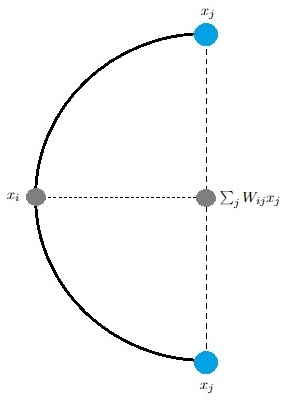
\includegraphics[width=\textwidth]{images/lle_illustraion.jpg}
         \caption{General illustration of the reconstruction.}
         \label{subfig:lle_illustraion}
     \end{subfigure}
     \hfill
     \begin{subfigure}[t]{0.40\textwidth}
         \centering
         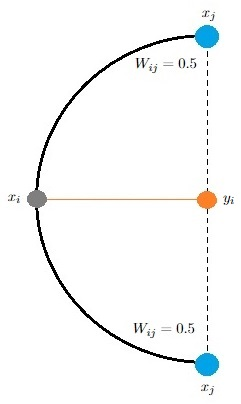
\includegraphics[width=\textwidth]{images/lle_0.5_0.5.jpg}
         \caption{Both contribute equally to the reconstruction of \textcolor{embedding}{$y_i$}.}
         \label{subfig:lle_0.5_0.5}
     \end{subfigure}
     \hfill
     \begin{subfigure}[t]{0.40\textwidth}
         \centering
         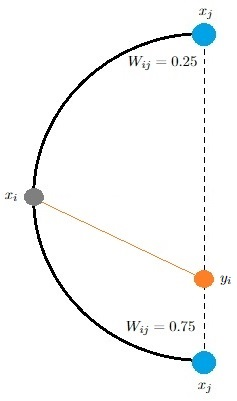
\includegraphics[width=\textwidth]{images/lle_0.75_0.25.jpg}
         \caption{One neighbor contributes more and the other one less to the reconstruction of \textcolor{embedding}{$y_i$}.}
         \label{subfig:lle_0.75_0.25}
     \end{subfigure}
     \hfill
     \begin{subfigure}[t]{0.40\textwidth}
         \centering
         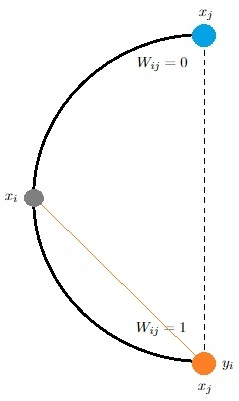
\includegraphics[width=\textwidth]{images/lle_1_0.jpg}
         \caption{One neighbor contributes none and the other one everything to the reconstruction of \textcolor{embedding}{$y_i$}.}
         \label{subfig:lle_1_0}
     \end{subfigure}
        \caption[How LLE reconstructs embeddings]{Own illustration on how LLE reconstructs embedding \textcolor{embedding}{$y_i$} with the help of the weights $W_{ij}$ from the neighbors \textcolor{neighbor}{$x_j$} from the input \textcolor{input}{$x_i$} based on Fig. 3 and Fig. 4 in \cite{saul03}}
        \label{fig:lle_illustration}
\end{figure}

\subsection{t-Distributed Stochastic Neighbor Embedding (t-SNE)}

The method "t-Distributed Stochastic Neighbor Embedding" (t-SNE) proposed by Maaten and Hinton in 2008 \cite{t-SNE08} originates from the "Stochastic Neighbor Embedding" (SNE) method proposed by Hinton and Roweis in 2002. \cite{SNE02} The t-SNE method is an upgrade to SNE that differs in two major aspects that will be discussed later in this paragraph. Both are considered statistical methods that work by creating \textit{probability distributions} around points in the original space and then trying to match distributions on the corresponding points in the embedded space by optimizing a cost function. Those probability distributions between points $x_i$ and $x_j$ in the original space are defined as
\begin{equation}
    p_{j|i}=\frac{e^{{-\norm{x_i-x_j}^2 / 2\sigma_i^2}}}{\sum_{k\neq i}e^{-\norm{x_i-x_k}^2 / 2\sigma_i^2}},
\end{equation}
represent similarities between points. For the prior distance measurement, the Euclidean distance is used. If those points that are compared are close to each other, then the probability that they can be considered neighbors is high, and if the points are far apart, then the probability that they are neighbors is low. Note that $p_{j|i}$ is normalized by dividing by the probability distribution of all points compared to $x_i$. This means that the probability distribution for a point sums up to 1, showed by the following equation
\begin{equation}
    \sum_j p_{j|i}=1.
\end{equation}
Another important aspect is that $p_{i|i}=0$ because we just want to consider pairwise similarities. The distribution that is fit onto $x_i$ in the original space is the \textit{Gaussian distribution}. Since the conditional probability is not symmetric, meaning $p_{j|i} \neq p_{i|j}$, t-SNE uses the mean of both probabilities
\begin{equation}
    p_{ij}=\frac{p_{j|i}+p_{i|j}}{2D},
\end{equation}
where D is the dimensionality of the original space $\mathbb{R}^D$. It is not symmetric because both points lie on different spots with different neighbors and therefore have different probability distributions. The use of the mean is the first differing aspect compared to SNE, where this step is not considered, resulting in a more difficult optimization task. Furthermore, t-SNE is a parametric method that needs a so-called \textit{perplexity} parameter. This parameter determines how the variance $\sigma_i$ of the Gaussian for a point is set because there is no single optimal value for it due to differing densities of regions. The best values are the ones that stretch the Gaussian so far that so many neighbors are in a reasonable probability range. To find the values for the different variance values, t-SNE performs a binary search algorithm regarding the perplexity parameter. An illustration of how the Gaussian changes with different $\sigma_i$ values is shown in Fig. \ref{fig:t-sne_sigma}. The perplexity for a probability distribution $P_i$ is defined as
\begin{equation}
    Perp(P_i)= 2^{-\sum_j p_{j|i} \log_2p_{j|i}}
\end{equation}
and in addition, the authors recommend a parameter range of 5 to 50 to obtain good results.
\begin{figure}[!]
	\centering
	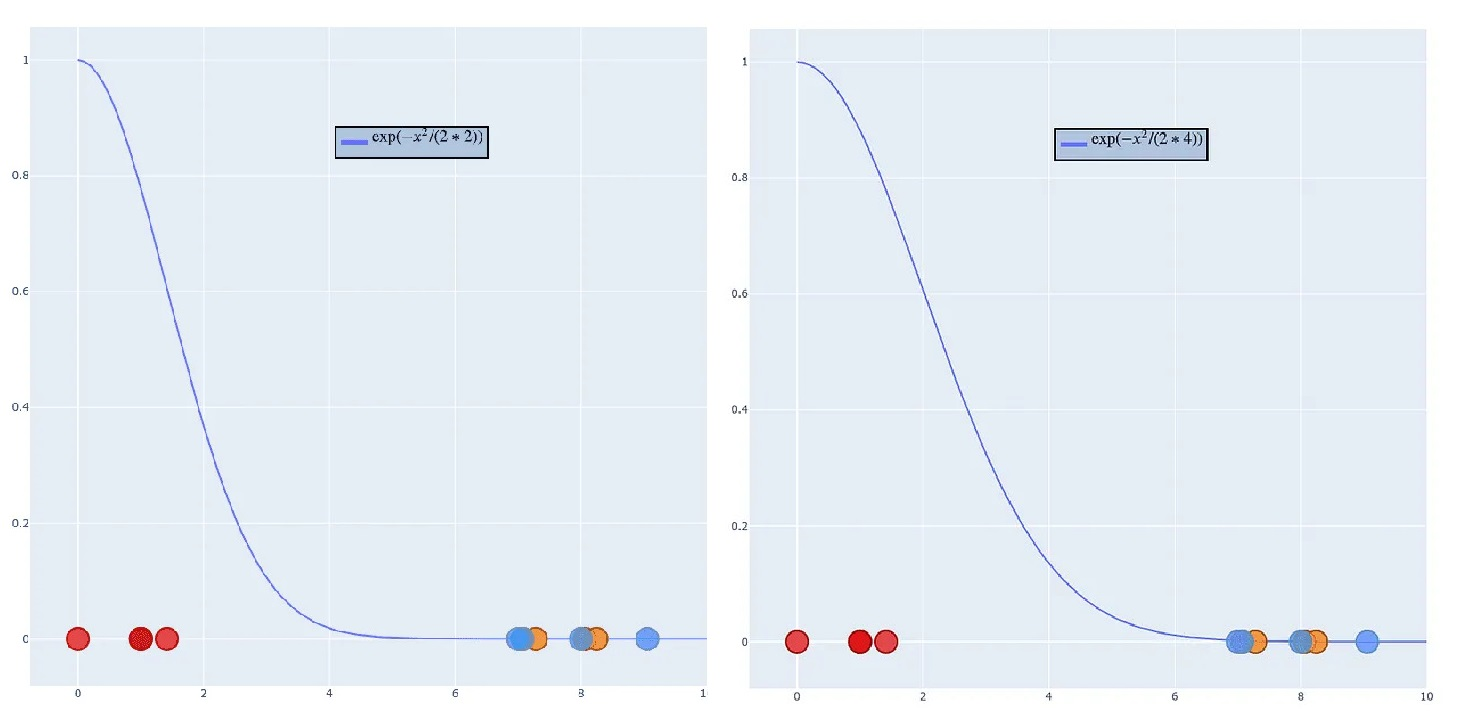
\includegraphics[width=\columnwidth]{images/t-sne_sigma.jpg}
	\caption[t-SNE difference in perplexity and therefore sigma]{Illustration of how the distribution curve changes with differing $\sigma_i$ values resulting from different perplexity parameters. On the left $\sigma_i=\sqrt{2}$ and on the right $\sigma_i=\sqrt{4}$. Adapted from $^2$.}
    \label{fig:t-sne_sigma}
\end{figure}
In the next step, the low dimensional probability distributions
\begin{equation}
    q_{ij}=\frac{(1+\norm{y_i-y_j}^2)^{-1}}{\sum_{k\neq l (1+\norm{y_i-y_k}^2)^{-1}}}
\end{equation}
that are also symmetric are searched for. For this purpose, instead of fitting a Gaussian again as in SNE, t-SNE uses a Student-t distribution with the advantage of having a "long" or "heavy tail". This prevents the so-called \textit{crowding problem}, which we will elaborate on in the next section.
\begin{figure}[!]
	\centering
	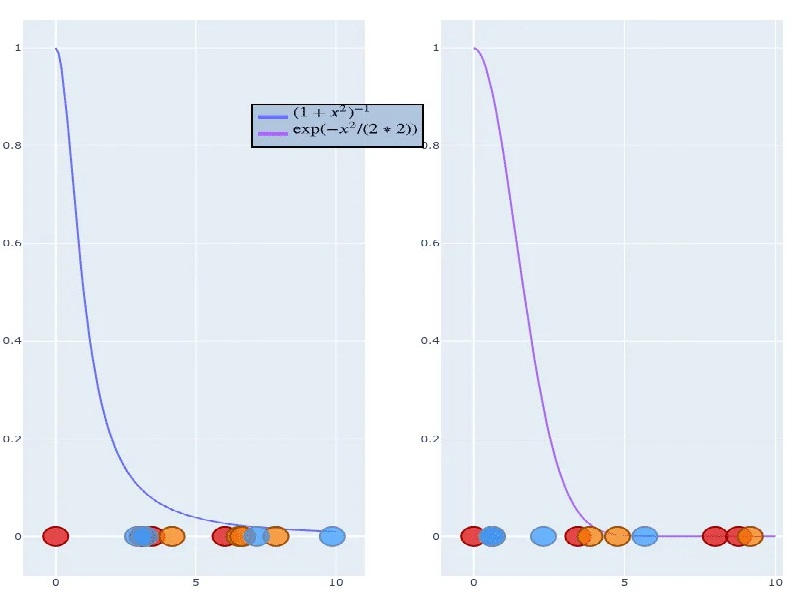
\includegraphics[width=\columnwidth]{images/t-sne_dists.jpg}
	\caption[t-SNE different distributions]{Illustration on how the distribution curves change by using Student-t (left) and Gaussian (right). Adapted from $^2$.}
    \label{fig:t-sne_dists}
\end{figure}
\footnotetext{\url{https://towardsdatascience.com/t-sne-clearly-explained-d84c537f53a}}
To find the low dimensional probability distributions, the following \textit{Kullback-Leibler divergence} 
\begin{equation}
    KL(P||Q)= \sum_i \sum_j p_{ij} \log \frac{p_{ij}}{q_{ij}}
\end{equation}
is minimized where $P$ is the \textit{joint probability distribution} in high dimensional space and $Q$ is the same in low dimensional space. This divergence simply calculates the difference between two probability distributions. However, it puts emphasis on matching high $p{ij}$ values with high $q{ij}$ values. If $p{ij}$ is low, the divergence does not penalty high $q{ij}$ values. Hence, t-SNE mainly preserves local similarity structures of the data. The optimization of the Kullback-Leibler divergence is performed by using \textit{gradient descent}. \cite{Gisbrecht15}

\subsection{Limitations}

Now that we have introduced some methods for learning a manifold, we want to address the limitation and disadvantages of such methods, also considering general restrictions of nonlinear dimensionality reduction.

\subsubsection{Computational Complexity}

One major drawback of NLDR methods is their high computational complexity, meaning they need more time to complete a computation or more memory storage to save intermediate results. The complexity is also much higher compared to LDR methods. This is due to the fact that they are designed to capture nonlinear relations of datasets and therefore are more complex. Especially when dealing with large datasets, the need for many computational resources is asked, which we also saw in Section \ref{sec:speed_and_accuracy}, where the computation of LLE could not be finished on some datasets. This fact also applies to t-SNE. This makes them less practical and sometimes infeasible for some applications with limited computational resources. [\cite{Zubova18}, \cite{t-SNE08}]

\subsubsection{Necessity of Parameter-Tuning} \label{subsubsec:parameter_tuning}

This limitation does not apply to the non-parametric MDS method but to the two other methods: LLE with its neighborhood-size parameter and t-SNE with its perplexity parameter. Those methods need parameter-tuning because different optimal parameter choices might exist for different datasets. These parameters can have a significant impact on the results. It is to be considered that an appropriate parameter grows with the overall number of points or the number of points in clusters. Therefore multiple runs with different choices are needed to find suitable parameters. An illustration of t-SNE with different perplexity values resulting in significantly differing visualizations is shown in Fig. \ref{fig:parameter-tuning}. [\cite{t-SNE08}, \cite{how_t-SNE16}]
\begin{figure}[!]
	\centering
	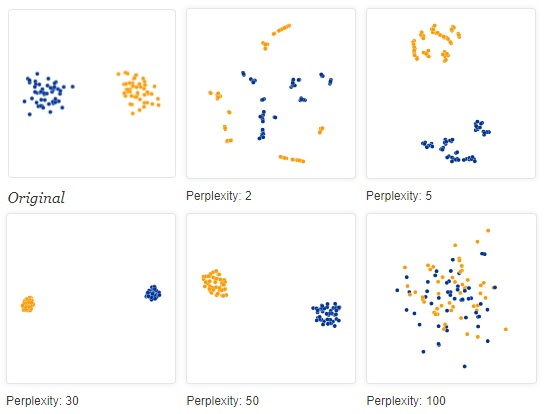
\includegraphics[width=0.9\columnwidth]{images/parameter-tuning.jpg}
	\caption[Impact of Parameters]{Illustration of how the perplexity parameter from t-SNE impacts the result, adapted from \footnotemark}
    \label{fig:parameter-tuning}
\end{figure}
\footnotetext{\url{https://distill.pub/2016/misread-tsne/}}

\subsubsection{Stuck in Local Minima}

The local minima problem applies to t-SNE because its computation is non-deterministic. The other two methods are deterministic, which means that for a fixed parameter, they have one single solution. Therefore non-deterministic means that the results can vary, although the input parameter did not change. This is because t-SNE uses gradient descent with random initialization to find a minimum. Finding a global minimum would be optimal, but in reality, the methods often get stuck in local minima. This makes it challenging to achieve consistent and reliable results over several attempts, especially by taking into consideration that we also need to tune the parameter of t-SNE. An illustration is shown in Fig. \ref{fig:local_minima}. \cite{t-SNE08}
\begin{figure}[!]
	\centering
	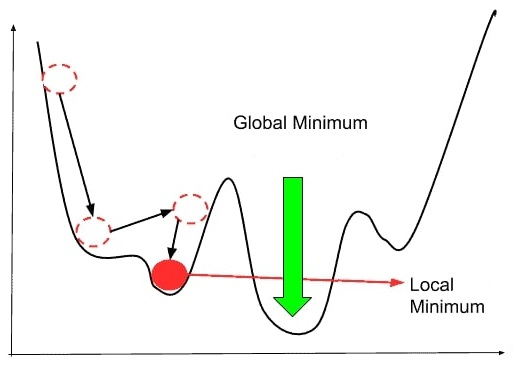
\includegraphics[width=0.7\columnwidth]{images/local_minima.jpg}
	\caption[Stuck in Local Minima]{Illustration of how gradient descent can get stuck in a \textcolor{red}{local minimum}. The finding of the \textcolor{green}{global minimum} would be optimal. Adapted from \footnotemark}
    \label{fig:local_minima}
\end{figure}
\footnotetext{\url{https://www.mltut.com/stochastic-gradient-descent-a-super-easy-complete-guide/}}

\subsubsection{Unknown Intrinsic Dimensionality}

So far, we haven't mentioned that another parameter must be set before computation for all methods. This parameter is the dimension of the low dimensional space to which we want to reduce the dataset. By reducing a dataset to some dimensionality, information might get lost. This is the case if the intrinsic dimensionality of the dataset is higher than the dimensionality we want to reduce to. For data visualization tasks, the potential loss of information is accepted because the dimensionality must be 3 or lower. For tasks that have the purpose of enhancing the analysis of a dataset, it is favorable if the intrinsic dimensionality matches the dimension of the embedded space so that the analysis is improved and no information got lost. An instance where information got lost because the reduction went further than the capable intrinsic dimensionality can be seen in Fig. \ref{fig:mds_illustration}, where the reduction to a 1-dimensional space could not preserve all pairwise distances.

\subsubsection{Short-Circuiting} \label{subsubsec:short}

Short-circuiting is the problem that occurs when multiple folds of a manifold are close to each other. If this happens, it is possible that one point from a fold falsely classifies another from the other fold as its neighbor, although they should not be considered neighbors at all. An illustration is shown in Fig. \ref{fig:short-circuit}. This happens because the Euclidean distance measure is used in high dimensional space. This metric does not take the curvature of manifolds into account. A better solution would be to use the \textit{Geodesic distance}. This metric measures the shortest paths or distances between points along the manifold. The difference between these measures can be seen in Fig. \ref{fig:Geodesic-versus-Euclidean}. This miss classification of neighbors can significantly alter the manifold's true topology, resulting in not bad but incorrect embeddings. This problem naturally occurs in MDS, where all pairwise distances are measured via Euclidean. However, in LLE and t-SNE, this problem can be countered by setting the parameters that determine the neighborhood sizes lower so that opposite lying folds can not be reached anymore. [\cite{short_circuit(1)}, \cite{short_circuit(2)}, \cite{geo_vs_eucl}]
\begin{figure}[!]
     \centering
     \begin{subfigure}[t]{0.55\columnwidth}
    	\centering
    	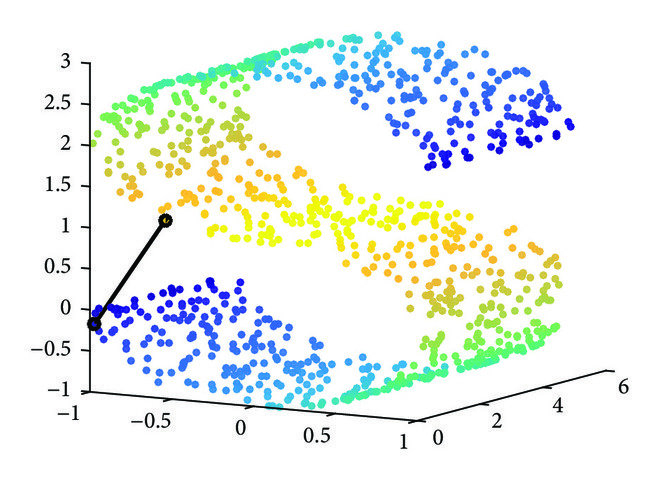
\includegraphics[width=\columnwidth]{images/short-circuit.jpg}
    	\caption{Short-Circuiting on an S-Curve dataset, adapted from \cite{short-circuit_fig}}
        \label{fig:short-circuit}
    \end{subfigure}
     \hfill
     \begin{subfigure}[t]{0.44\columnwidth}
    	\centering
    	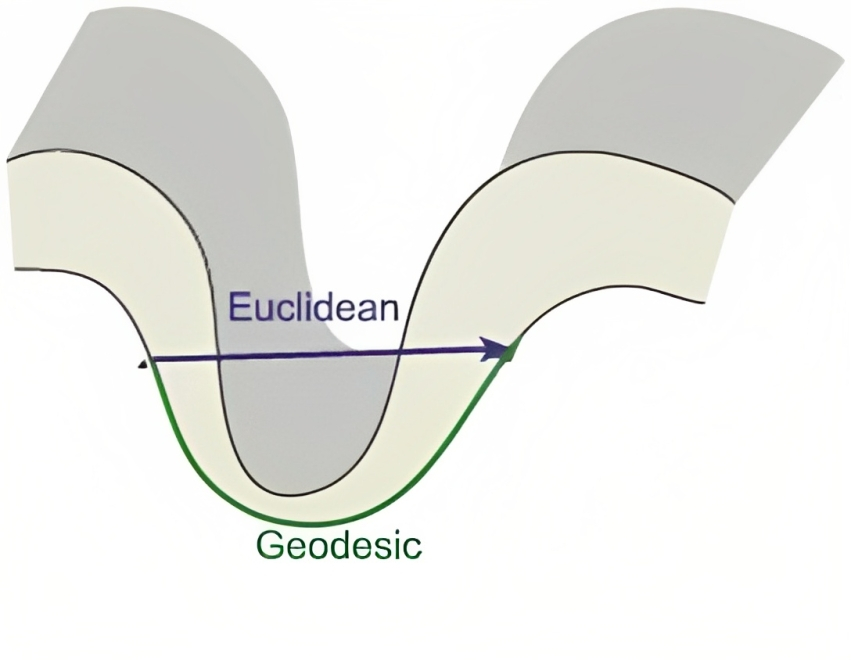
\includegraphics[width=\columnwidth]{images/Geodesic-versus-Euclidean.jpg}
    	\caption{\textcolor{geodesic}{Geodesic} vs. \textcolor{euclidean}{Euclidean} distance, adapted from \cite{geo_vs_eucl}}
        \label{fig:Geodesic-versus-Euclidean}
    \end{subfigure}
     \caption[Problem of Short-Circuiting]{Illustration of the Short-Circuiting Problem}
    \label{fig:problem_short-circuiting}
\end{figure}

\subsubsection{Global vs. Local}

It is important to understand that it is always a trade-off between preserving more global or more local structures of datasets. Preserving local structure means that neighbors are placed accurately, but non-neighbors may be much closer or farther away than the original manifold. It seems that local methods can handle sharp curvatures better than global methods. MDS, for example, is a global structure preserving method and cannot be tweaked to emphasize local patterns. LLE and t-SNE, however, can change the emphasis with different parameter settings. Although one can increase the parameters, this can lead to the previously mentioned short-circuiting problem. Too low values can result in entirely leaving out the global structure. It can, for example, happen that coherent regions in the original space are torn apart in the embedded space. So one must find a balance between global and local preserving needs. An illustration of how the visualization changed with parameters is shown in Fig. \ref{fig:mammoth}. [\cite{Cayton05}, \cite{mammoth}]
\begin{figure}[!]
	\centering
	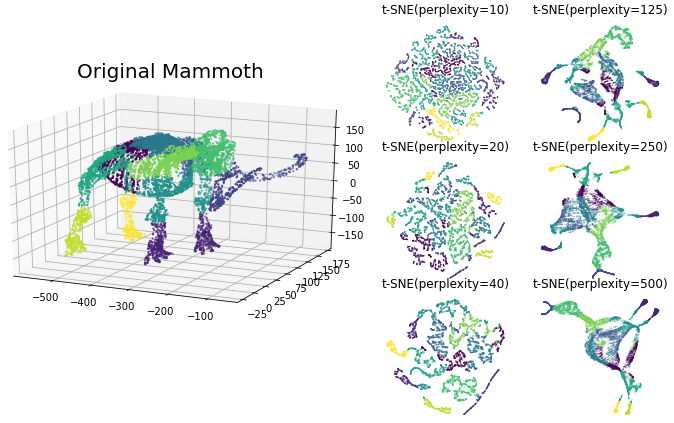
\includegraphics[width=1\columnwidth]{images/mammoth.jpg}
	\caption[Global vs. Local Structures]{Illustration of how the perplexity affects the emphasis of global or local structure. The higher the perplexity, the more the global structure (shape of the mammoth) is preserved. Adapted from Fig. 1 in \cite{mammoth}}
    \label{fig:mammoth}
\end{figure}

\subsubsection{Crowding Problem} \label{subsubsec:crowding}

The crowding problem is a problem that occurs when trying to reduce a high dimensional dataset with 
also a high intrinsic dimensionality to a lower dimensionality. In this case, the reduction results in a compressed or, in the worst case, collapsed manifold. To understand why this happens, one must understand that the space volume is proportional to the number of dimensions, meaning the higher the dimension, the larger the space (Fig. \ref{fig:crowding_problem}). If we now want to reduce this number of dimensions, the points that initially had plenty of space now need to arrange themselves in a much smaller space. This especially happens to LLE, where point clouds collapse into single points, and some outlier points are used to fulfill the constraints of the cost function. However, t-SNE overcomes this issue using a Student-t distribution instead of the Gaussian distribution for the embedded space. This enables the placement of moderately distant points to be placed further apart. One can think of stretching the manifold in the low dimensional space. [\cite{t-SNE08}, \cite{Gisbrecht15}]
\begin{figure}[!]
	\centering
	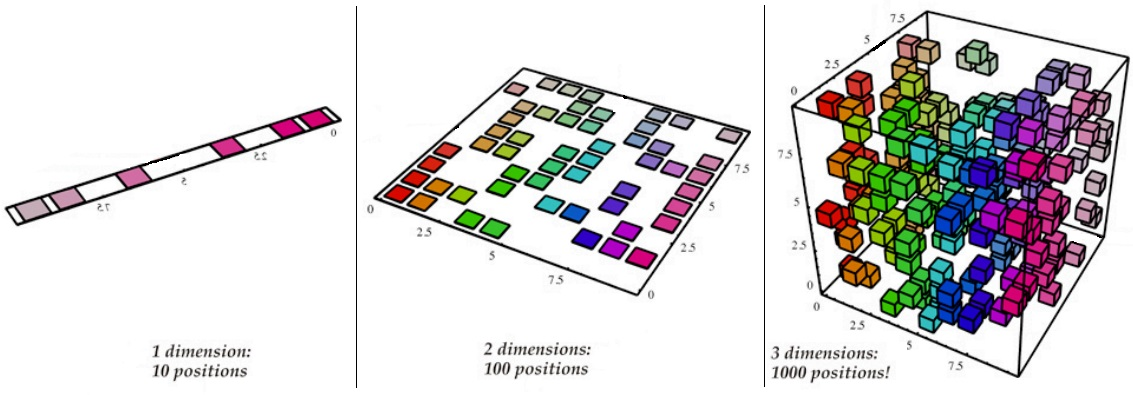
\includegraphics[width=1\columnwidth]{images/crowding_problem.jpg}
	\caption[Crowding Problem]{Illustration of how the space increases with dimensions and the points that can fit into it. Adapted from \footnotemark}
    \label{fig:crowding_problem}
\end{figure}
\footnotetext{\url{https://pub.towardsai.net/a-probabilistic-algorithm-to-reduce-dimensions-t-distributed-stochastic-neighbor-embedding-23ff457fbc8a}}

\subsubsection{Interpretability}

By applying DR methods to datasets, we get a low dimensional representation of this data. But this is not the end of the story, we also need to interpret these results. This can be done by either objective or subjective measures. Objective measures, which we will elaborate on in Chapter \ref{cap:methodology}, are measures where no two opinions exist. Subjective measures, however, are used in visualization tasks and heavily rely on the sight of the human eye. Moreover, no two pairs of eyes are alike and let alone the brain that is connected to them, resulting in, in the worst case, significantly different perceptions of the same thing. In addition to that, low dimensional visualizations do not always convey meaning. This can be seen in the example of t-SNE. The resulting cluster sizes most often do not mean anything because the method adapts its notion of distances to regional densities instead of a global notion. "As a result, it naturally expands dense clusters, and contracts sparse ones, evening out cluster sizes." \cite{how_t-SNE16} (Fig. \ref{fig:t-sne_density}) A similar phenomenon holds for clusters that are not equidistantly distributed, which should be preserved in the embedding. But t-SNE places these clusters somehow equidistantly. (Fig. \ref{fig:t-sne_cluster_distances}) \cite{how_t-SNE16}
\begin{figure}[!]
     \centering
     \begin{subfigure}[t]{0.9\columnwidth}
    	\centering
    	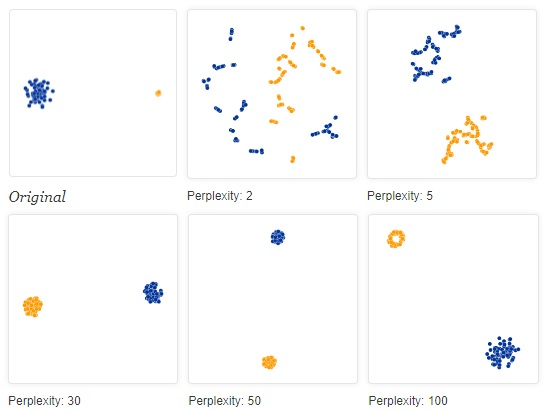
\includegraphics[width=1\columnwidth]{images/t-sne_density.jpg}
    	\caption{Evening out cluster densities}
        \label{fig:t-sne_density}
    \end{subfigure}
     \hfill
     \begin{subfigure}[t]{0.9\columnwidth}
    	\centering
    	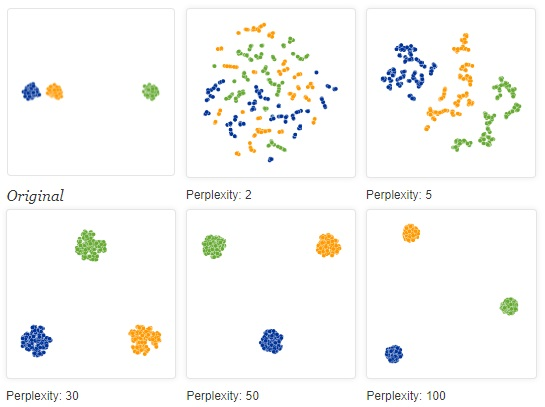
\includegraphics[width=\columnwidth]{images/t-sne_cluster_distances.jpg}
    	\caption{Evening out cluster distances}
        \label{fig:t-sne_cluster_distances}
    \end{subfigure}
     \caption[Interpretability of t-SNE]{Illustration of the restricted interpretability of t-SNE, adapted from $^5$}
    \label{fig:t-sne_interpret}
\end{figure}

\subsubsection{Unrealistic Assumptions}

Manifold learning as a whole comes with many assumptions, which is quite normal because it is not possible to portray the world's complexity even closely. That's why it needs to simplify things and set assumptions so that the computational complexity does not explode. In addition, every method has its own assumptions that come on top of the existing ones. It is important to note that these assumptions are not always accurate for all datasets. The success of manifold learning techniques depends on how well the data conform to these assumptions. In some cases, it may be necessary to modify the techniques or pre-process the data to account for violations of these assumptions.

\paragraph{Low dimensional manifold that lies in high dimensional space} is the first major assumption manifold learning has. This assumption is often motivated by the observation that many high dimensional datasets exhibit a low dimensional structure that can be uncovered through dimensionality reduction. This is, for example, not true for cases where intrinsic dimensionality equals the extrinsic dimensionality of the dataset. \cite{Cayton05}

\paragraph{Manifolds are locally linear} is another assumption that states that a linear mapping between the high dimensional and low dimensional spaces can approximate the local structure of a manifold. This assumption is especially crucial when a sparse dataset is given where the point that are considered neighbors by the method are actually far apart where a Geodesic distance would result in a better outcome. \cite{t-SNE08}

\paragraph{Manifolds are uniform and continuous} (Fig. \ref{fig:uniform_manifold}) is an assumption that is always invalid for real-world data. It states that the density of data points is roughly constant, and data points are coherent across the manifold. This assumption is important for LLE, where there needs to be sufficient data points in each local neighborhood to estimate the local structure of the manifold accurately. Therefore, LLE performs weakly on datasets with multiple widely separated, maybe not connected, sub-manifolds because the constructed neighborhood graph is not connected adequately. \cite{t-SNE08}
\begin{figure}[!]
	\centering
	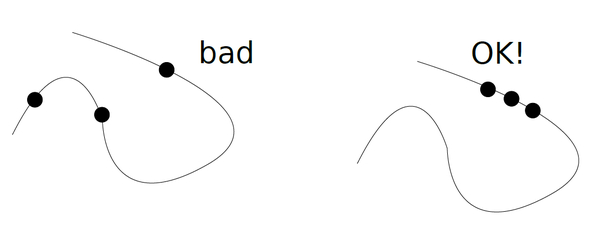
\includegraphics[width=1\columnwidth]{images/uniform_manifold.jpg}
	\caption[Uniform and Continuous Manifold]{Illustration of OK! (right) and bad (left) point densities on a manifold, adapted from \footnotemark}
    \label{fig:uniform_manifold}
\end{figure}
\footnotetext{\url{https://www.quora.com/What-are-the-limitations-of-manifold-learning}}

\paragraph{Distances/similarities are symmetric} is a valid assumption from a mathematical standpoint, but it might be that point $x_i$ is more similar to $x_j$ than $x_j$ to $x_i$. The predecessor of t-SNE did not apply this assumption, leading to a more complex optimization step but, counterintuitively, a weaker performance. \cite{t-SNE08}

\section{Clustering Algorithms} \label{sec:clustering}

The following section is needed to understand the concepts of clustering and clustering algorithms. In our experiments, we will need the latter to form clusters in the embedded space of our high dimensional datasets and evaluate the clustering performances. We will elaborate on what performance means in Chapter \ref{cap:methodology}. Before going into algorithms that complete the task of clustering, we introduce the notion of clustering. In clustering, we are interested in finding structure in unlabeled data, called unsupervised learning. More specifically, we are trying to group similar objects, which also leads to separating dissimilar ones. There are multiple types of such clustering algorithms. Some are hierarchical, grid-based, model-based, partitional, and density-based clustering. We will only elaborate on the last two types, where we will also introduce the associated algorithms $k$-means and DBSCAN, respectively. The crucial difference between those is that $k$-means will find convex-shaped clusters that are primarily spherical or elliptical. Whereas DBSCAN is not bound to any shapes and, therefore, can find arbitrary-shaped clusters. An illustration of that is shown in Fig. \ref{fig:dbscan_vs_k-means}.
\cite{clustering(1)}
\begin{figure}[!]
	\centering
	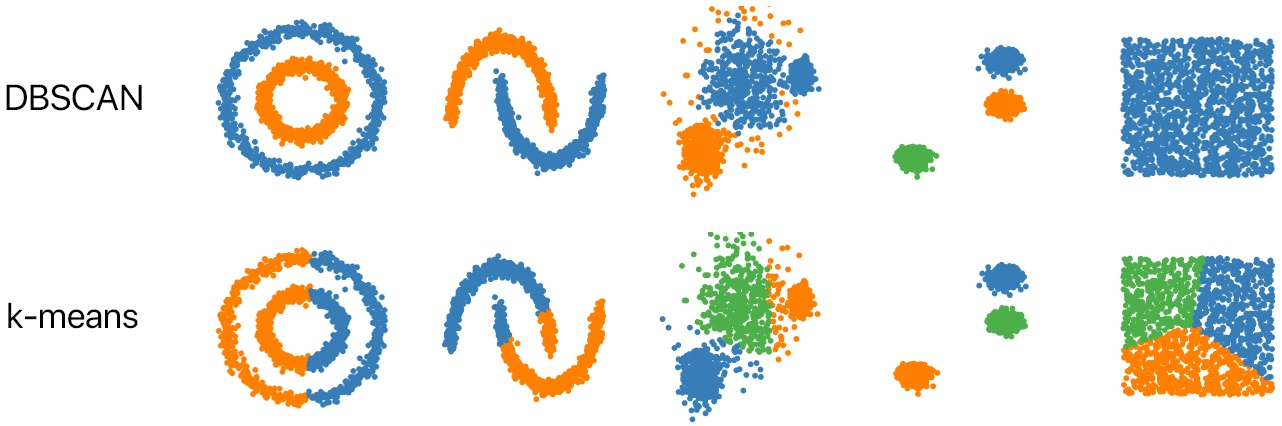
\includegraphics[width=1\columnwidth]{images/dbscan_vs_k-means.jpg}
	\caption[DBSCAN vs. $k$-means]{Illustration of how the shapes of the clusters are formed from DBSCAN (arbitrary) and $k$-means (convex). Adapted from \footnotemark}
    \label{fig:dbscan_vs_k-means}
\end{figure}
\footnotetext{\url{https://user-images.githubusercontent.com/7659/74451662-d2325000-4e34-11ea-9770-a57e81259eb9.png}}

\subsection{k-Means} \label{k-means}

K-means is a clustering algorithm that works in an iterative manner, and in each iteration, it refines the clustering results to better ones. The algorithms need the parameter $k$ to be set, which fixes the number of clusters to be found. This is also the major drawback of this algorithm, as we need to know the $k$ before computation which is unrealistic if we do not have a domain expert or a visual representation of the dataset. In the following, we will describe the functionality of $k$-means in four steps, which are visually demonstrated in Fig. \ref{fig:k-means}: 1. Initially place $k$ center points, called centroids, randomly 2. Assign each point to its closest centroid where Euclidean distance is used 3. Set new centroid positions to the average of all points in the specific clusters 4. Repeat steps 2. and 3. until no changes in centroid positions emerge, also called convergence. K-means is a prevalent algorithm because it is computationally not very intensive, and its implementation is straightforward. Those advantages, however, do come with significant disadvantages. One of which is that, again, the parameter $k$ must be set prior to computation, and also it is sensitive to outliers. Another one is that its computation is non-deterministic because it can get stuck in local minima. The initialization of the centroid also has an impact on the resulting cluster. [\cite{clustering(1)}, \cite{wiki_k-means}]
\begin{figure}[!]
	\centering
	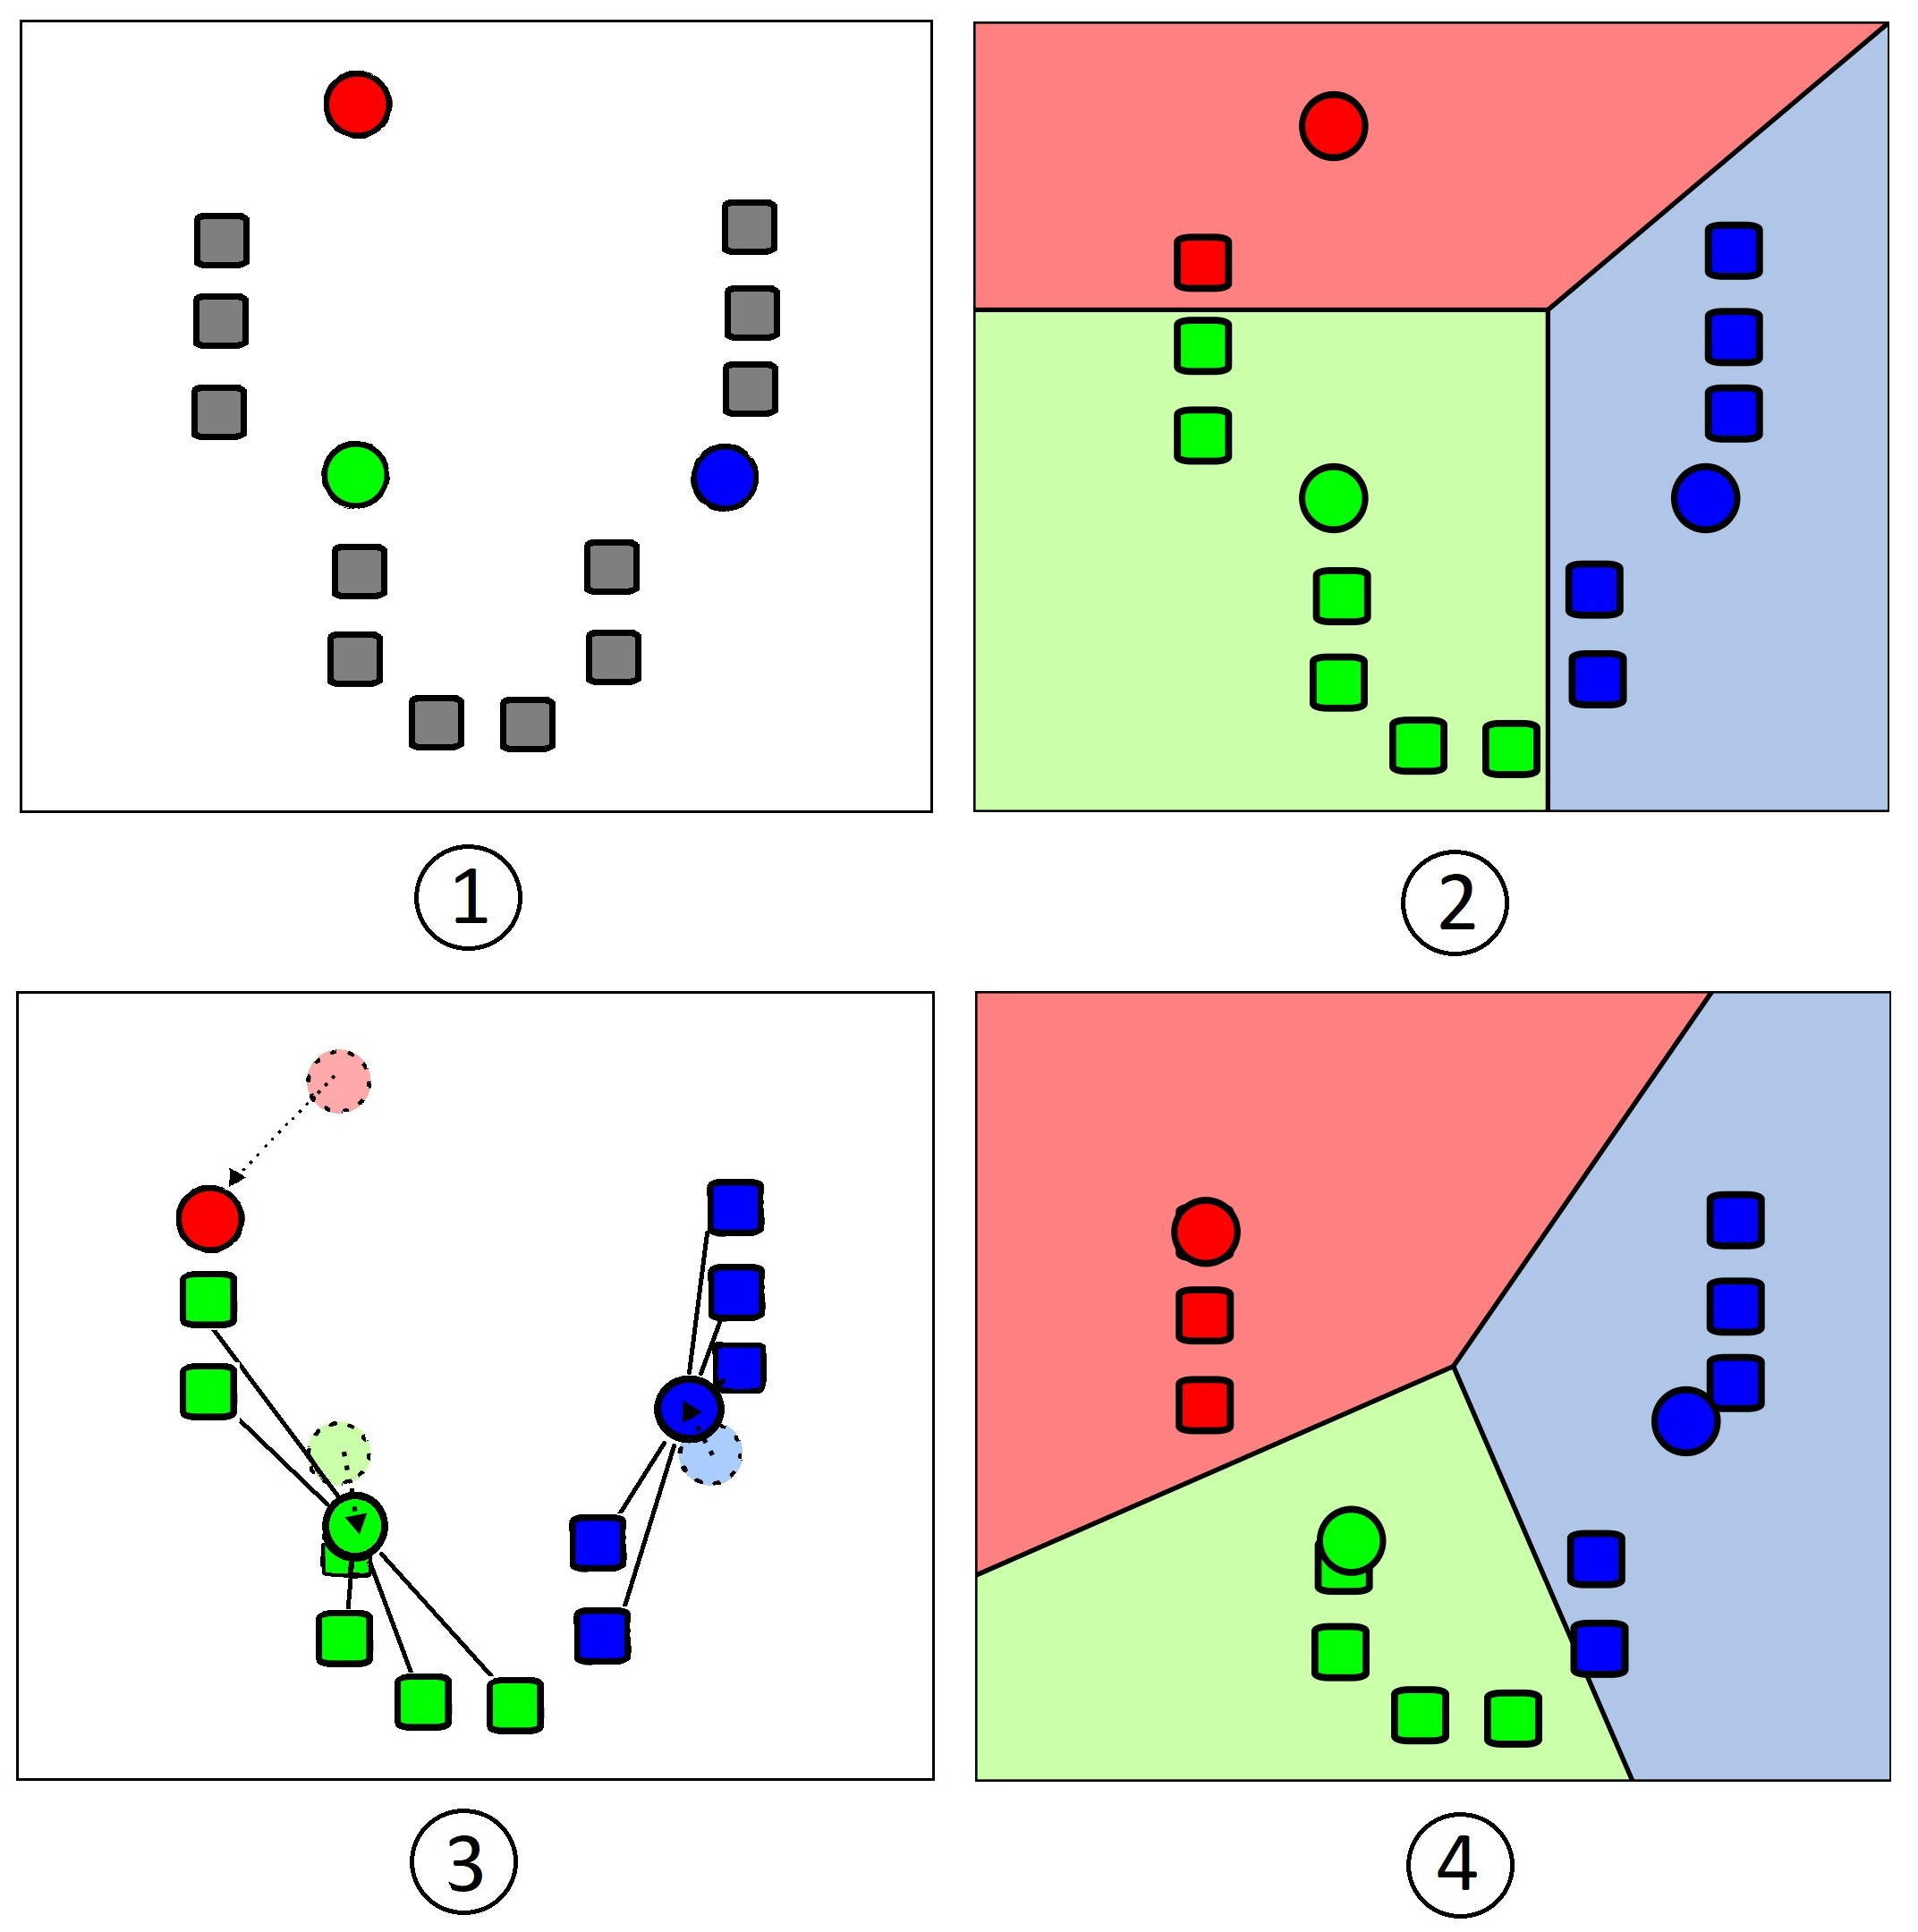
\includegraphics[width=0.75\columnwidth]{images/k-means.jpg}
	\caption[Illustration of $k$-Means]{Illustration of $k$-means where the steps correspond to the steps described in Sec. \ref{k-means}, adapted from \cite{wiki_k-means}}
    \label{fig:k-means}
\end{figure}

\subsection{DBSCAN}

The clustering algorithm DBSCAN which stands for \textit{Density Based Spatial Clustering of Applications with Noise}, is a density-based clustering technique. The clusters are identified by defining a density via the parameters set by the user and then assigning points to either core, border, or noise points. (Fig. \ref{fig:dbscan}) The parameters that have to be set are $Eps$ and $MinPts$. The algorithm then starts by selecting a point from the dataset and calculating the $Eps$-$neighborhood$ of this point. All points in the $Eps$-range, meaning that the distance to another point is lower or equal to $Eps$, are in the $Eps$-$neighborhood$. If the $Eps$-$neighborhood$ is higher or equal to $MinPts$, this point is classified as a core point, and the procedure is further applied to all points in the $Eps$-$neighborhood$. But if the $Eps$-$neighborhood$ is lower than $MinPts$, the point is classified as a border point. Suppose there are no further points to visit in the $Eps$-$neighborhood$. Another point is then selected, and the algorithm does the same to that point as to the initial point. This is done until all points are processed. The points that were reachable from a core point are considered a cluster. All other points that do not belong to clusters are classified as noise points. Note that border points can join clusters but not extend them. The authors emphasize that DBSCAN is suited for large datasets with noise and that knowing the number of clusters is unnecessary, which is a huge advantage of $k$-means. However, a major disadvantage of this method is that it cannot handle datasets with varying densities well because the parameters define a global notion of density. Furthermore, as we don't know the best parameter setting, the utilization of parameter tuning is necessary. However, this is not easy because DBSCAN is non-deterministic and depends on the initialization. [\cite{clustering(1)}, \cite{dbscan}]
\begin{figure}[!]
	\centering
	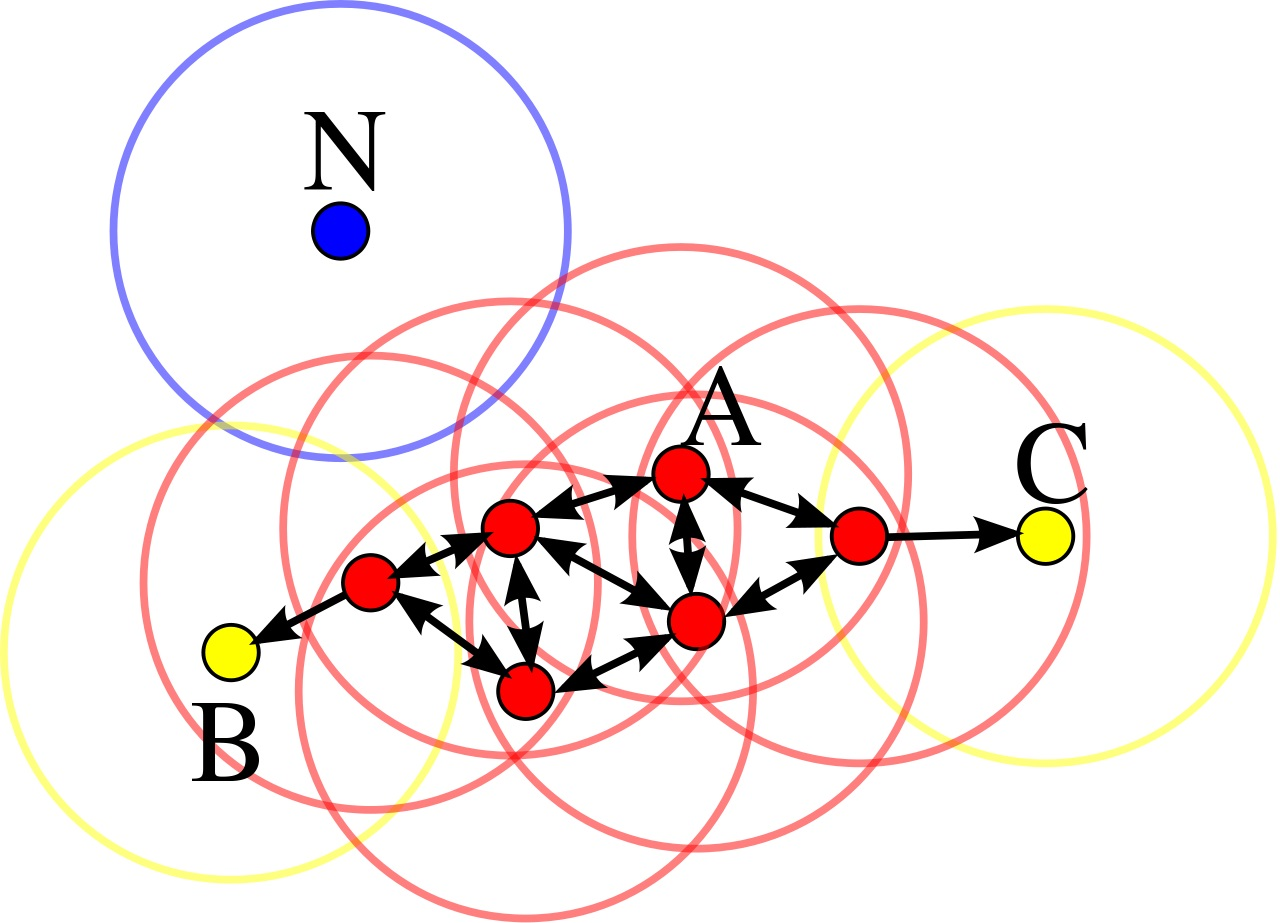
\includegraphics[width=0.75\columnwidth]{images/dbscan.jpg}
	\caption[Illustration of DBSCAN]{Illustration of DBSCAN where \textcolor{red}{core}, \textcolor{yellow}{border} and \textcolor{blue}{noise} points are depicted. Adapted from \footnotemark}
    \label{fig:dbscan}
\end{figure}
\footnotetext{\url{https://commons.wikimedia.org/wiki/File:DBSCAN-Illustration.svg}}
